% Define important features for the document
\documentclass[12pt,oneside]{article}
\setlength{\parindent}{0pt}
\setlength{\parskip}{4pt}

% Import packages
\usepackage[margin = 1in]{geometry}
\usepackage{amsfonts, amsmath, amssymb, amsthm, calc, centernot, color, csquotes, dsfont, enumitem, environ, fancyhdr, fontawesome5, graphicx, hyperref, marvosym, mathrsfs, mathtools, tcolorbox, titlesec}
\usepackage[flushmargin,hang]{footmisc}
\tcbuselibrary{breakable}

% Define toggles
\newif\ifsolutions
\solutionstrue % Toggle for instructor version
% \solutionsfalse % Toggle for student version

% Define size and spacing of section and subsection
\titleformat{\section}
  {\normalfont\large\bfseries}
  {\thesection}{1em}{}
\titleformat{\subsection}
  {\normalfont\normalsize\bfseries}
  {\thesubsection}{1em}{}
\titlespacing*{\section}{0pt}{6pt}{6pt} % ({left}{before}{after})
\titlespacing*{\subsection}{0pt}{6pt}{6pt} % ({left}{before}{after})

% Define commands
\newcommand{\indep}{\perp\!\!\!\perp}
\newcommand{\notindep}{\mathrel{\not\!\perp\!\!\!\perp}}
\newcommand{\E}{\mathbb{E}}
\newcommand{\Var}{\text{Var}}
\newcommand{\Cov}{\text{Cov}}
\newcommand{\Corr}{\text{Corr}}
\newcommand{\SD}{\text{SD}}
\newcommand{\SE}{\text{SE}}
\newcommand{\Bias}{\text{Bias}}
\newcommand{\MSE}{\text{MSE}}
\newcommand{\Risk}{\text{Risk}}
\newcommand{\Like}{\mathcal{L}}
\newcommand{\boot}{\text{boot}}
\newcommand{\strat}{\text{strat}}
\newcommand{\supp}{\text{supp}}
\newcommand{\MLE}{\text{MLE}}
\newcommand{\MoM}{\text{MoM}}
\newcommand{\MOM}{\text{MOM}}
\newcommand{\OLS}{\text{OLS}}
\newcommand{\LS}{\text{LS}}
\newcommand{\MAP}{\text{MAP}}
\newcommand{\MAE}{\text{MAE}}
\newcommand{\LP}{\text{LP}}
\newcommand{\HT}{\text{HT}}
\newcommand{\JS}{\text{JS}}
\newcommand{\RB}{\text{RB}}
\newcommand{\UB}{\text{UB}}
\newcommand{\DIM}{\text{DIM}}
\newcommand{\PATE}{\text{PATE}}
\newcommand{\SATE}{\text{SATE}}
\newcommand{\VIF}{\text{VIF}}
\newcommand{\GVIF}{\text{GVIF}}
\newcommand{\AIC}{\text{AIC}}
\newcommand{\BIC}{\text{BIC}}
\newcommand{\LASSO}{\text{LASSO}}
\newcommand{\PSS}{\text{PSS}}
\newcommand{\CV}{\text{CV}}
\newcommand{\logit}{\text{logit}}
\newcommand{\odds}{\text{odds}}
\newcommand{\OR}{\text{OR}}
\newcommand{\N}{\mathcal{N}}
\newcommand{\Bern}{\text{Bern}}
\newcommand{\Bin}{\text{Bin}}
\newcommand{\Beta}{\text{Beta}}
\newcommand{\Gam}{\text{Gamma}}
\newcommand{\Expo}{\text{Expo}}
\newcommand{\Pois}{\text{Pois}}
\newcommand{\Unif}{\text{Unif}}
\newcommand{\DUnif}{\text{DUnif}}
\newcommand{\Geom}{\text{Geom}}
\newcommand{\FS}{\text{FS}}
\newcommand{\NBin}{\text{NBin}}
\newcommand{\HGeom}{\text{HGeom}}
\newcommand{\Mult}{\text{Mult}}
\newcommand{\MVN}{\text{MVN}}
\newcommand{\IG}{\text{IG}}
\newcommand{\Tweedie}{\text{Tweedie}}
\newcommand{\simiid}{\overset{\text{i.i.d.}}{\sim}}
\newcommand{\simind}{\overset{\text{ind.}}{\sim}}
\newcommand{\simnull}{\overset{H_0}{\sim}}
\newcommand{\simapprox}{\overset{\cdot}{\sim}}
\newcommand{\R}{\mathbb{R}}
\newcommand{\Z}{\mathbb{Z}}
\newcommand{\Q}{\mathbb{Q}}
\newcommand{\C}{\mathbb{C}}
\newcommand{\I}{\mathbb{I}}
\newcommand{\indic}{\mathds{1}}
\newcommand{\iid}{\text{i.i.d.}}
\newcommand{\Ind}{\text{Ind}}
\newcommand{\SSq}{\text{SSq}}
\newcommand{\trace}{\text{trace}}
\newcommand{\rank}{\text{rank}}
\newcommand{\diag}{\text{diag}}
\newcommand{\adj}{\text{adj}}
\newcommand{\SSE}{\text{SSE}}
\newcommand{\SST}{\text{SST}}
\newcommand{\SSR}{\text{SSR}}
\newcommand{\GLS}{\text{GLS}}
\newcommand{\ti}{\text{time}}
\newcommand{\outcome}{\text{outcome}}
\newcommand{\exposure}{\text{exposure}}
\newcommand{\NA}{\text{NA}}
\newcommand{\cp}{\text{cp}}
\newcommand{\tip}{\textbf{\faLightbulb}: }
\newcommand{\warning}{\textbf{\Biohazard}: }
\newcommand{\blank}[1][4cm]{\underline{\hspace{#1}}}

% Define theorem-style environment (italic body, bold header)
\newtheorem{theorem}{Theorem}
\newtheorem{lemma}{Lemma}
\newtheorem{proposition}{Proposition}
\newtheorem{corollary}{Corollary}

% Define definition-style environment (upright body, bold header)
\theoremstyle{definition}
\newtheorem{definition}{Definition}
\newtheorem{example}{Example}
\newtheorem{problem}{\faPen \ Problem}
\newtheorem{concept}{\faPen \ Concept Checker}
\newtheorem{challenge}{\faFire \ Challenge}
\newtheorem{activity}{\faDiceThree \ Activity}

% Define idea-style environment (unnumbered definition)
\newtheorem*{idea}{Idea}

% Define remark-style environment (upright body, italic header)
\theoremstyle{remark}
\newtheorem{remark}{Remark}

% Define environment for solution box
\newsavebox{\solutioncontentbox}
\NewEnviron{solutionbox}[1][Solution]{
  \sbox{\solutioncontentbox}{
    \begin{minipage}{\dimexpr\linewidth-2\fboxsep\relax}
      \BODY
    \end{minipage}
  }
  \ifsolutions
    \begin{tcolorbox}[
      title=#1,
      colback=gray!5,
      colframe=black,
      breakable
    ]
      \BODY
    \end{tcolorbox}
  \else
    \begin{tcolorbox}[
      title=#1,
      colback=white,
      colframe=black,
      breakable,
      height=\dimexpr\ht\solutioncontentbox+\dp\solutioncontentbox+1cm\relax
    ]
    \end{tcolorbox}
  \fi
}

% Begin document
\begin{document}
\pagestyle{fancy}
\fancyhead[L]{STAT 110: Introduction to Probability}
\fancyhead[R]{Fall 2026}
\begin{center}
\bf \Large
Section 3: Random Variables \\[0.5em]
\normalsize
Avery Kim (\href{mailto:averykim@college.harvard.edu}{\texttt{averykim@college.harvard.edu}}), \\[0.2em]
Ricky Truong (\href{mailto:rickytruong@college.harvard.edu}{\texttt{rickytruong@college.harvard.edu}})
\end{center}

% Section: Introduction
\section{Introduction}

\subsection{Logistics}

Welcome! The goal of our weekly section is to review content from lecture, with emphasis on big-picture intuition, mathematical derivation, and hands-on practice.

Specifically, we aim for section to be interactive, well-paced, inclusive, and fun! Please do not hesitate to reach out if you have any questions/feedback!

\subsection{Office Hours}

$\bullet$ See the Google Calendar for the most accurate information!

\subsection{Attendance}

$\bullet$ \href{https://bit.ly/stat110harvard}{\texttt{bit.ly/stat110harvard}}

% Section: Random Variables
\section{Random Variables}

\begin{idea}
What will a stock price be tomorrow? What score will you get on the final exam? Life is full of unknown quantities, and \textit{random variables} allow us to better understand them by connecting everyday numbers with concepts in \textit{probability}.
\end{idea}

\begin{center}
  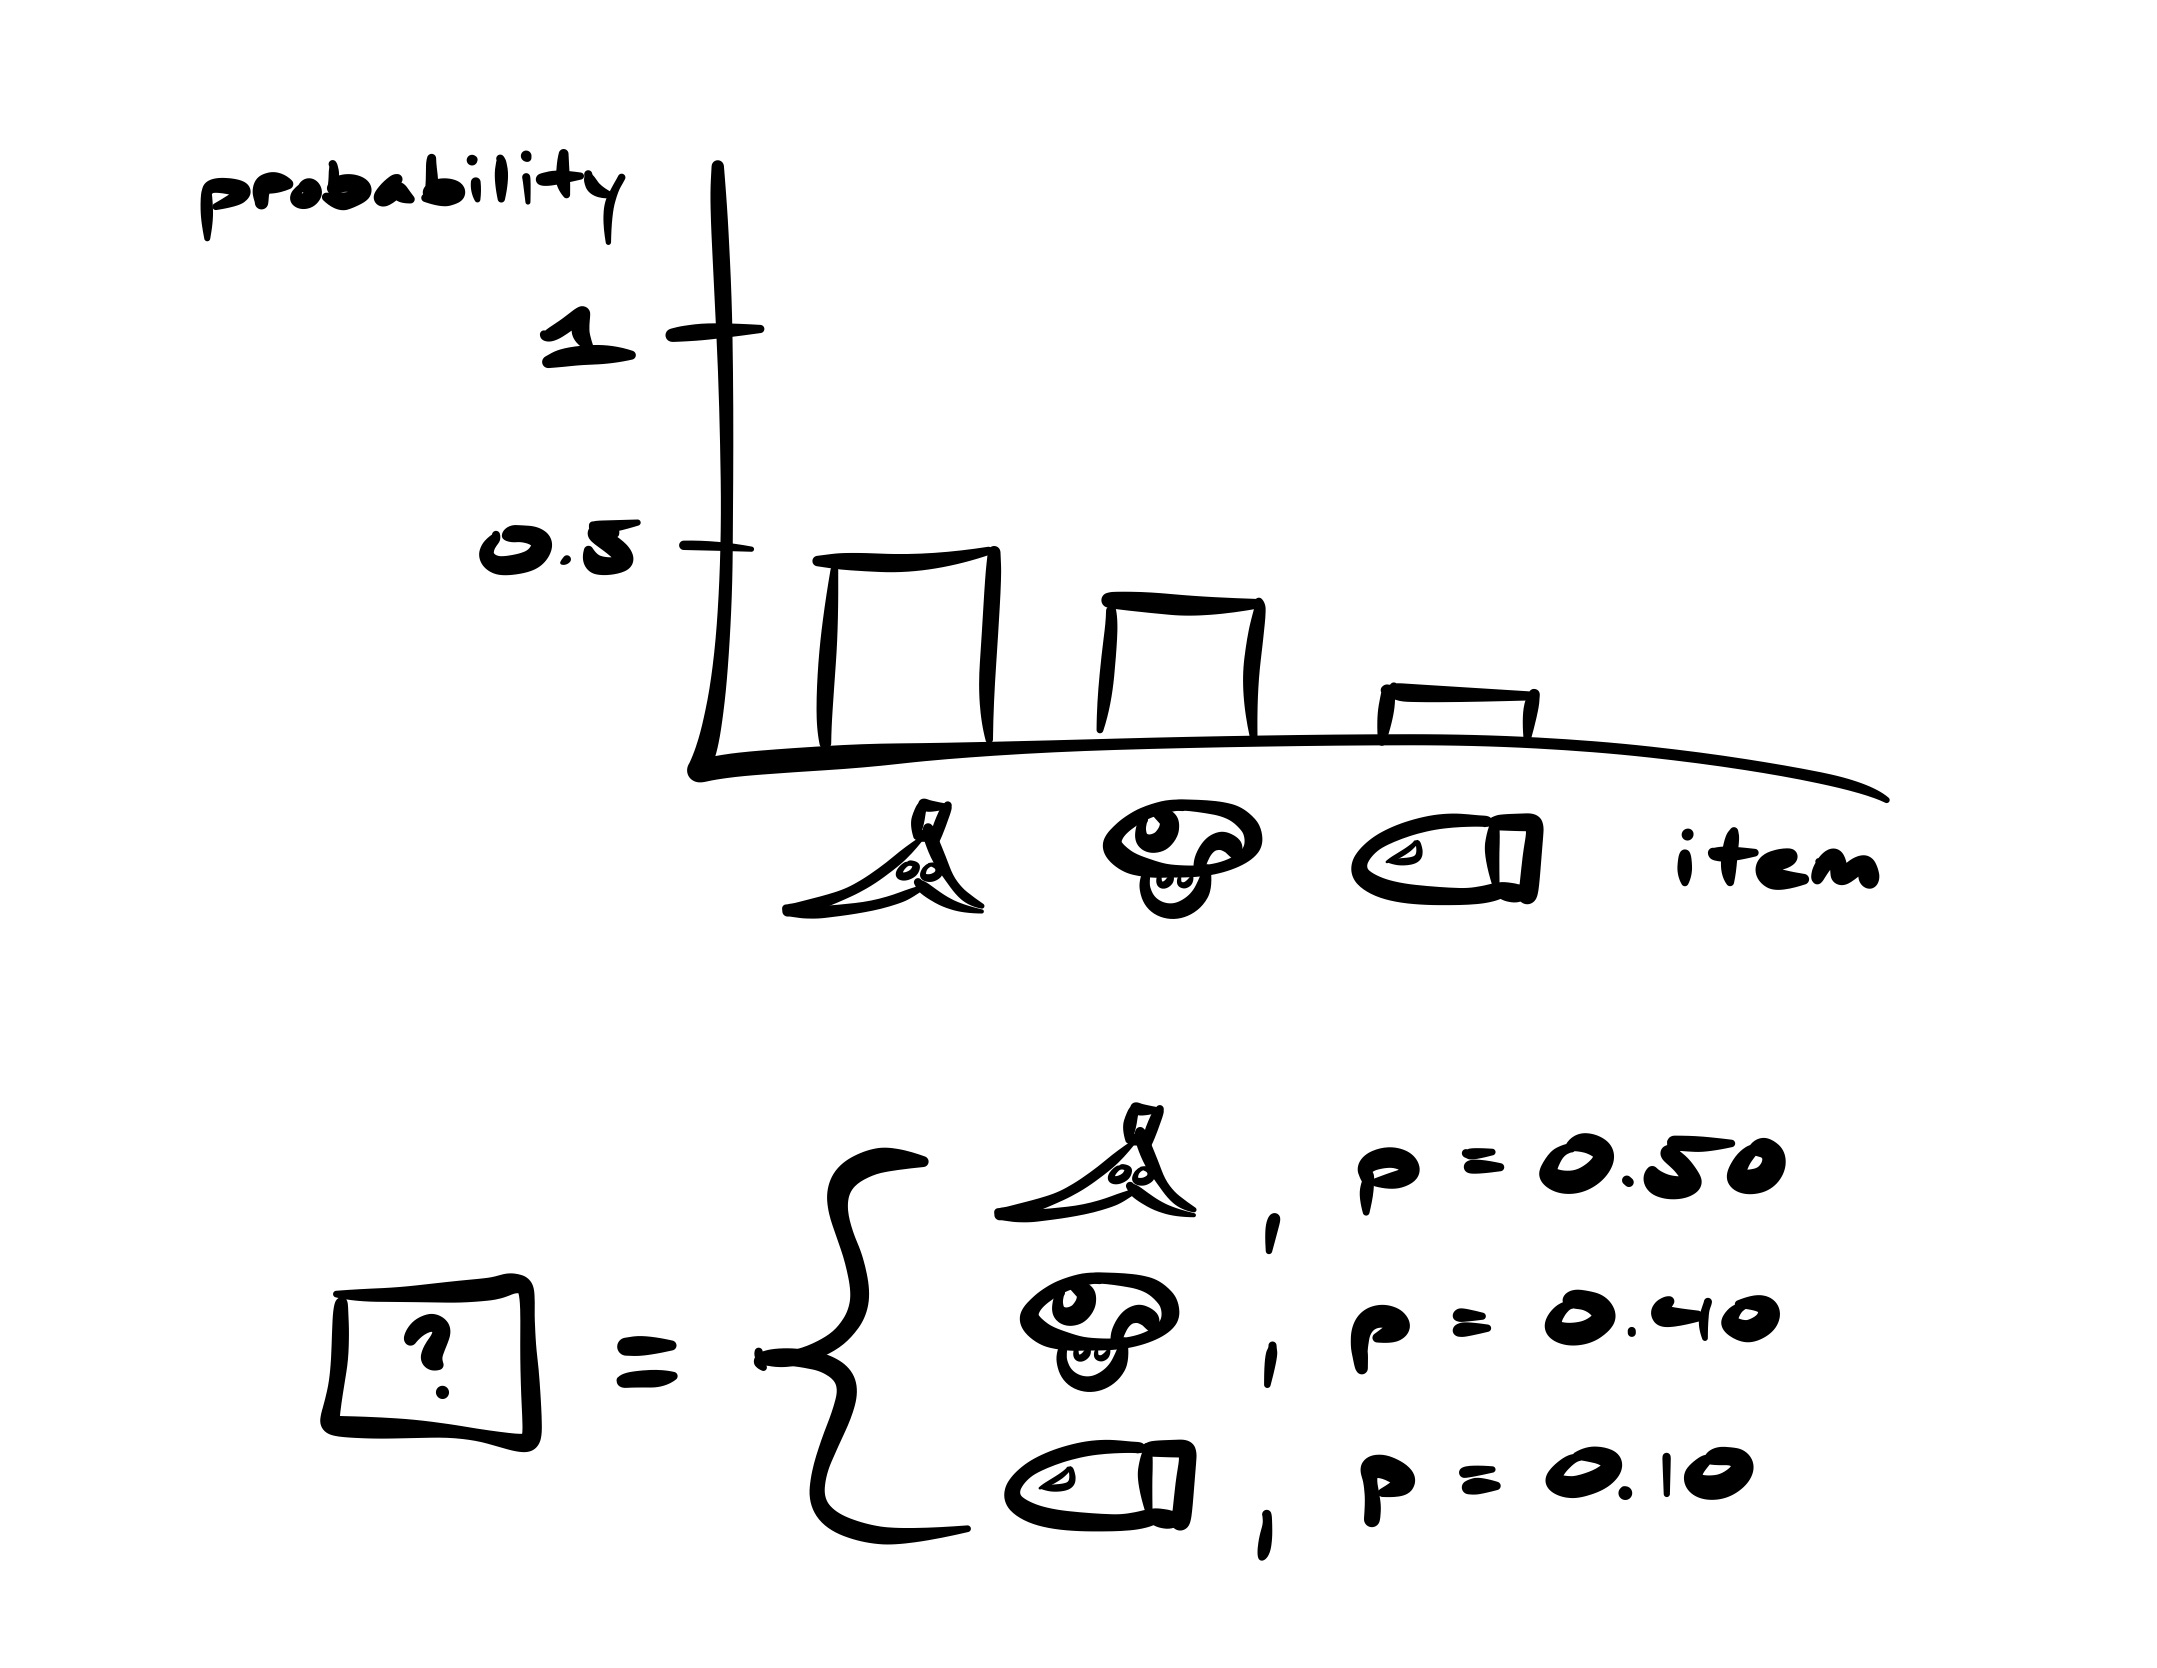
\includegraphics[width=0.5\textwidth]{stat110_section3_figure1.jpg}\\{\footnotesize FIGURE 1: The distribution of an item box in Mario Kart.}
\end{center}

\begin{definition}[Random variable]
Formally, a \textit{random variable} $X$ is a \textit{function} that assigns a real number to each possible outcome in the sample space.

$\bullet$ Informally, it is an unknown value that will \textit{crystallize} to some number after an experiment.

$\bullet$ \tip For some intuition, it is like an \textit{item box} in \textit{Mario Kart} (as illustrated in Figure 1)—it is unknown what value it will take on, but through its distribution, we can describe the possible values (along with which ones are more likely).
\end{definition}

\begin{center}
  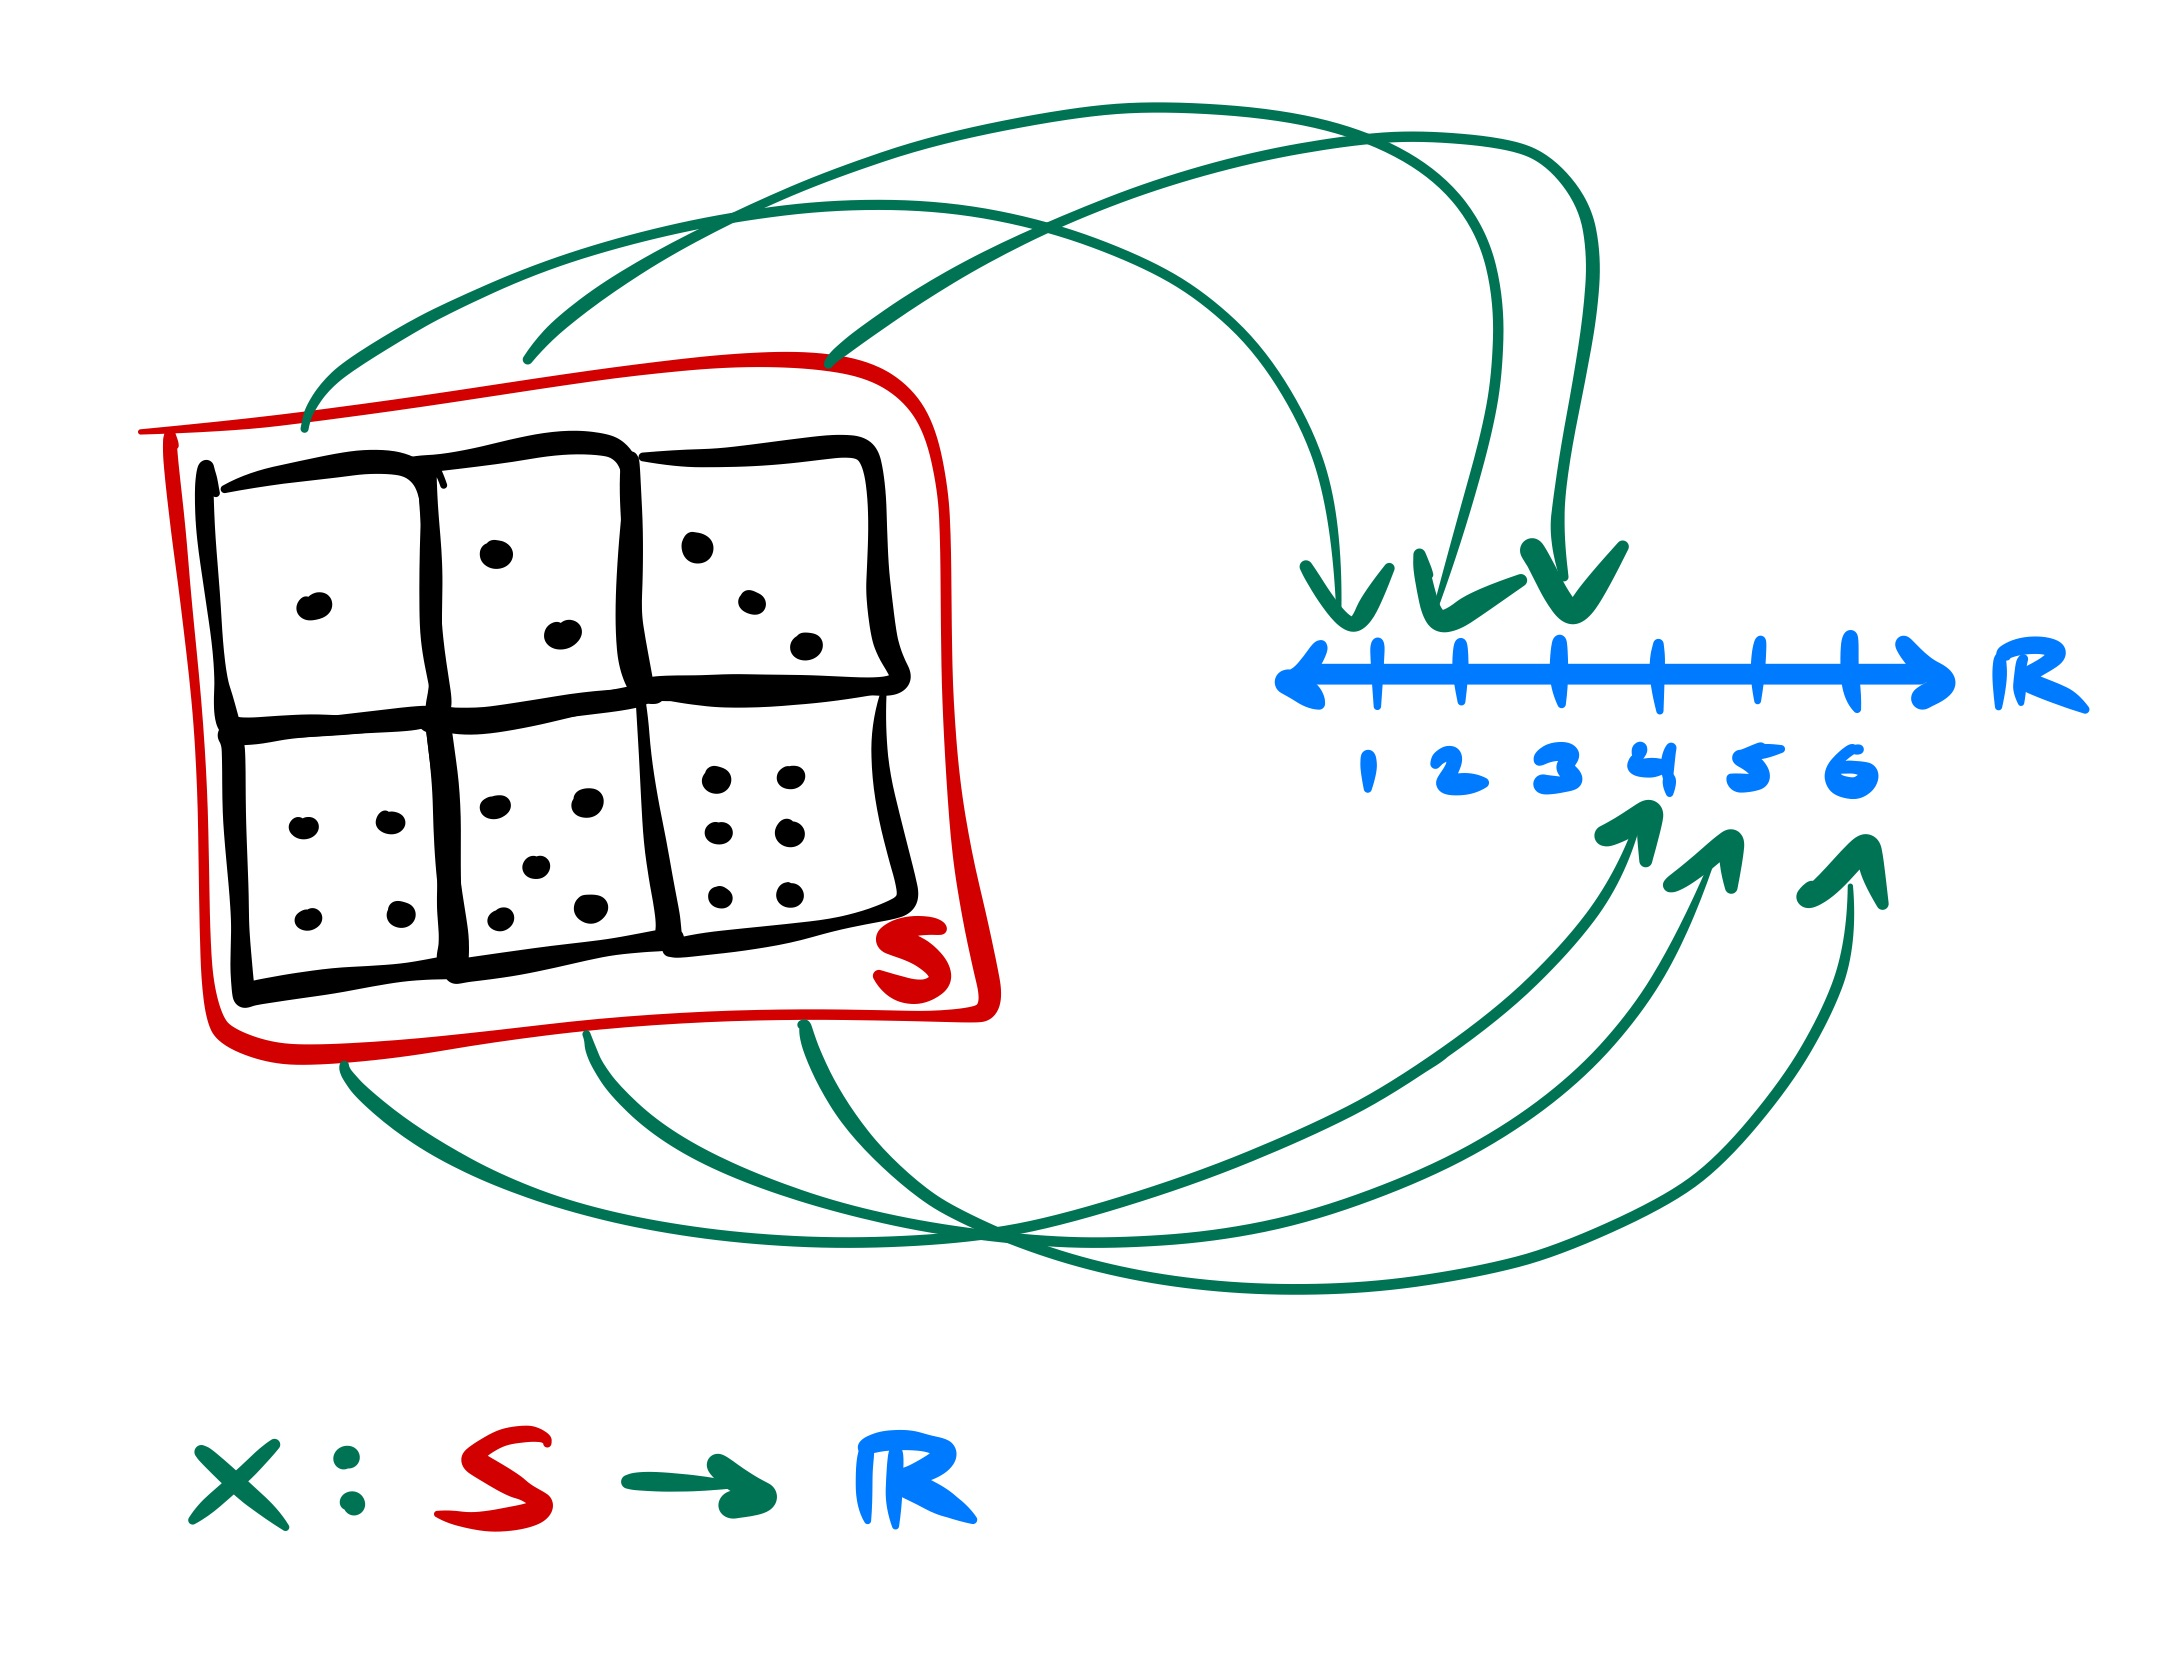
\includegraphics[width=0.5\textwidth]{stat110_section3_figure2.jpg}\\{\footnotesize FIGURE 2: The random variable $X$ maps each outcome in $S$ onto the number line.}
\end{center}

\begin{example}[Die roll as a random variable]
Let $X$ be the value of a fair die roll. There are $6$ outcomes in the sample space. As illustrated in Figure 2, each one is mapped to a real number.

$\bullet$ $\{\text{we roll a 1}\} \rightarrow 1, \{\text{we roll a 2}\} \rightarrow 2, \ldots, \{\text{we roll a 6}\} \rightarrow 6$.
\end{example}

\begin{definition}[Support]
The \textit{support} of a random variable $X$ is the set of all possible values $X$ can take on.

$\bullet$ $X$ is \textit{discrete} if its support is countable (or countably infinite) and \textit{continuous} otherwise.

$\bullet$ \tip Write down the support of all random variables you're working with. This will serve as a sanity check (and may even give you partial credit)!
\end{definition}

\begin{concept}
Suppose that we flip a fair coin $10$ times and let $X$ be the number of heads we observe. What is the support of $X$? What is $P(X = 10)$ (i.e., the probability that $X$ crystallizes to $10$)?
\end{concept}

\begin{solutionbox}
We could observe $0$ heads, $1$ head, and so on (up to all $10$ heads), so the support of $X$ is $\{0, 1, \ldots, 10\}$, which makes $X$ a discrete random variable. $P(X = 10) = (0.5)^{10}$.
\end{solutionbox}

\begin{definition}[Distribution]
The \textit{distribution} of a random variable $X$ specifies the probabilities of $X$ crystallizing to the values in its \textit{support}.

$\bullet$ Informally, it describes $X$—e.g., how likely is $\{X = 0\}$ vs. $\{X = 1\}$?

$\bullet$ \warning Random variable $\neq$ distribution. E.g., $\{X = 1\}$ is the event that $X$ crystallizes to 1 while $X \sim \Bern(0.5)$ describes the type of random variable $X$ is. 
\end{definition}

\begin{definition}[Probability mass function]
If a random variable $X$ is \textit{discrete}, then we can describe its distribution with $P(X = x)$, where $P(X = x)$ is the \textit{probability mass function} (PMF).

$\bullet$ A PMF for $X$ with support $\{x_1, x_2, \ldots\}$ must satisfy the following criteria:

$\bullet$ \textbf{Nonnegative}: $P(X = x) \geq 0$ for all $x$—i.e., probability cannot be negative.

$\bullet$ \textbf{Sums to 1}: $\sum_{i = 1}^{\infty} P(X = x_i) = 1$—i.e., all probabilities sum to 1 since $X$ must crystallize to something.
\end{definition}

\begin{concept}
Let $X$ be a discrete random variable with PMF $P(X = x)$. What is the PMF a function of?
\end{concept}

\begin{solutionbox}
The PMF is a function of possible crystallizations of $X$—e.g., $P(X = 0)$ vs. $P(X = 1)$. We denote an arbitrary crystallization as $x$ and say $P(X = x)$ is a function of $x$ (in the same way, e.g., $f(x) = x^2$ is a function of $x$). $X$ is the only thing that's random (and the randomness from $X$ comes from the experiment), but $P(X = x)$ is a probability and thus just a number.
\end{solutionbox}

% Section: Famous Distributions
\section{Famous Distributions}

\begin{idea}
Many random variables will match the \textit{story} of a \textit{famous distribution}, which will make our lives easier! If this happens, we can take advantage of the known properties and PMF. The challenge is often in recognizing the story/distribution and finding the parameters.
\end{idea}

\begin{definition}[Parameters]
To specify a \textit{distribution}, we must include its \textit{parameters} inside the parentheses.

$\bullet$ E.g., $X \sim \Bern(0.5)$ is different from $X \sim \Bern(0.7)$.
\end{definition}

\begin{definition}[Bernoulli]
Let $X$ be distributed \textit{Bernoulli} with parameter $p$—i.e., \[X \sim \Bern(p).\]

$\bullet$ \textbf{Story}: $X$ succeeds (i.e., $X = 1$) with probability $p$ and fails (i.e., $X = 0$) with probability $1 - p$.

$\bullet$ \textbf{Example}: Let $X = 1$ if a fair coin lands heads and $X = 0$ otherwise. Then $X \sim \Bern(0.5)$.

$\bullet$ \textbf{PMF and Support}: \[P(X = x) = p^x (1 - p)^{1 - x}\] for $x \in \{0, 1\}$.
\end{definition}

\begin{definition}[Indicator]
An \textit{indicator} for an event $A$ is a \textit{Bernoulli} random variable that equals 1 if $A$ occurs and 0 otherwise. 

$\bullet$ Formally, \[\indic\{A\} \sim \Bern(P(A)).\]
\end{definition}

\begin{definition}[Binomial]
Let $X$ be distributed \textit{Binomial} with parameters $n$ and $p$—i.e., \[X \sim \Bin(n, p).\]

$\bullet$ \textbf{Story}: $X$ is the number of successes in $n$ independent trials that each have success probability $p$.

$\bullet$ \textbf{Example}: Let $X$ be the number of heads observed if we flip a fair coin $10$ times. Then $X \sim \Bin(10, 0.5)$.

$\bullet$ \textbf{PMF and Support}: \[P(X = x) = \binom{n}{x} p^x (1 - p)^{n - x}\] for $x \in \{0, 1, \ldots, n\}$.

$\bullet$ \textbf{Properties}: If $X \sim \Bin(n, p)$ and $Y \sim \Bin(m, p)$ with $X \indep Y$, then \[X + Y \sim \Bin(n + m, p).\] If $X_1, \ldots, X_n \simiid \Bern(p)$, then \[X_1 + \ldots + X_n \sim \Bin(n, p).\]
\end{definition}

\begin{concept}
Let $X \sim \Bin(n, p)$ and $Y \sim \Bin(m, p)$ with $X \indep Y$. Show that $X + Y \sim \Bin(n + m, p)$ via story proof. Explain why $X - Y$ is not Binomial.
\end{concept}

\begin{solutionbox}
$X$ counts the number of successes in $n$ independent trials, and $Y$ counts the number of successes in $m$ independent trials (and all these trials have success probability $p$). Importantly, the trials in $X$ are independent of those in $Y$, so $X + Y$ counts the number of successes in $n + m$ independent trials (each with success probability $p$). By the story of the Binomial, $X + Y \sim \Bin(n + m, p)$. However, $X - Y$ cannot be Binomial since $X - Y$ can crystallize to negative values, which are outside the support of the Binomial.
\end{solutionbox}

% Section: More on Random Variables
\section{More on Random Variables}

\begin{idea}
We add more advanced concepts to everything we've discussed on random variables.
\end{idea}

\begin{definition}[Functions of random variables]
If $X$ is a random variable, then $Y = g(X)$ is \textit{also} a random variable for any function $g: \R \rightarrow \R$.

$\bullet$ If $g$ is a \textit{one-to-one} function, where the possible values of $X$ are $x_1, x_2, \ldots$ with respective probabilities $p_1, p_2, \ldots$, then the possible values of $Y$ are $g(x_1), g(x_2), \ldots$ with respective probabilities  $p_1, p_2, \ldots$ (i.e., $Y$ shares the same probabilities as $X$).

$\bullet$ E.g., if $X \sim \Bern(0.5)$ and $Y = 2X$, then $Y =
\begin{cases} 
    0, & p = 0.5 \\
    2, & p = 0.5 
\end{cases}$.
\end{definition}

\begin{definition}[Independence of random variables]
Random variables $X$ and $Y$ are \textit{independent} if \[P(X \leq x, Y \leq y) = P(X \leq x) P(Y \leq y)\] for all $x, y \in \R$.

$\bullet$ If $X \indep Y$, then $f(X) \indep g(Y)$ for any functions $f: \R \rightarrow \R$ and $g: \R \rightarrow \R$.

$\bullet$ E.g., let $X$ be the value of a fair die roll and $Y$ be the temperature tomorrow. Then $X \indep Y$.
\end{definition}

\begin{definition}[Independent and identically distributed]
Random variables $X$ and $Y$ are \textit{independent and identically distributed} (i.i.d.) if they are \textit{independent} and have the \textit{same distribution}—i.e., if $X \indep Y$ and $X, Y \sim F$ for some distribution $F$.

$\bullet$ E.g., suppose that we flip a fair coin 20 times. Let $X$ be the number of heads observed in the first 10 flips and $Y$ be the number of heads observed in the last 10 flips. Then $X, Y \simiid \Bin(10, 0.5)$.
\end{definition}

\begin{center}
  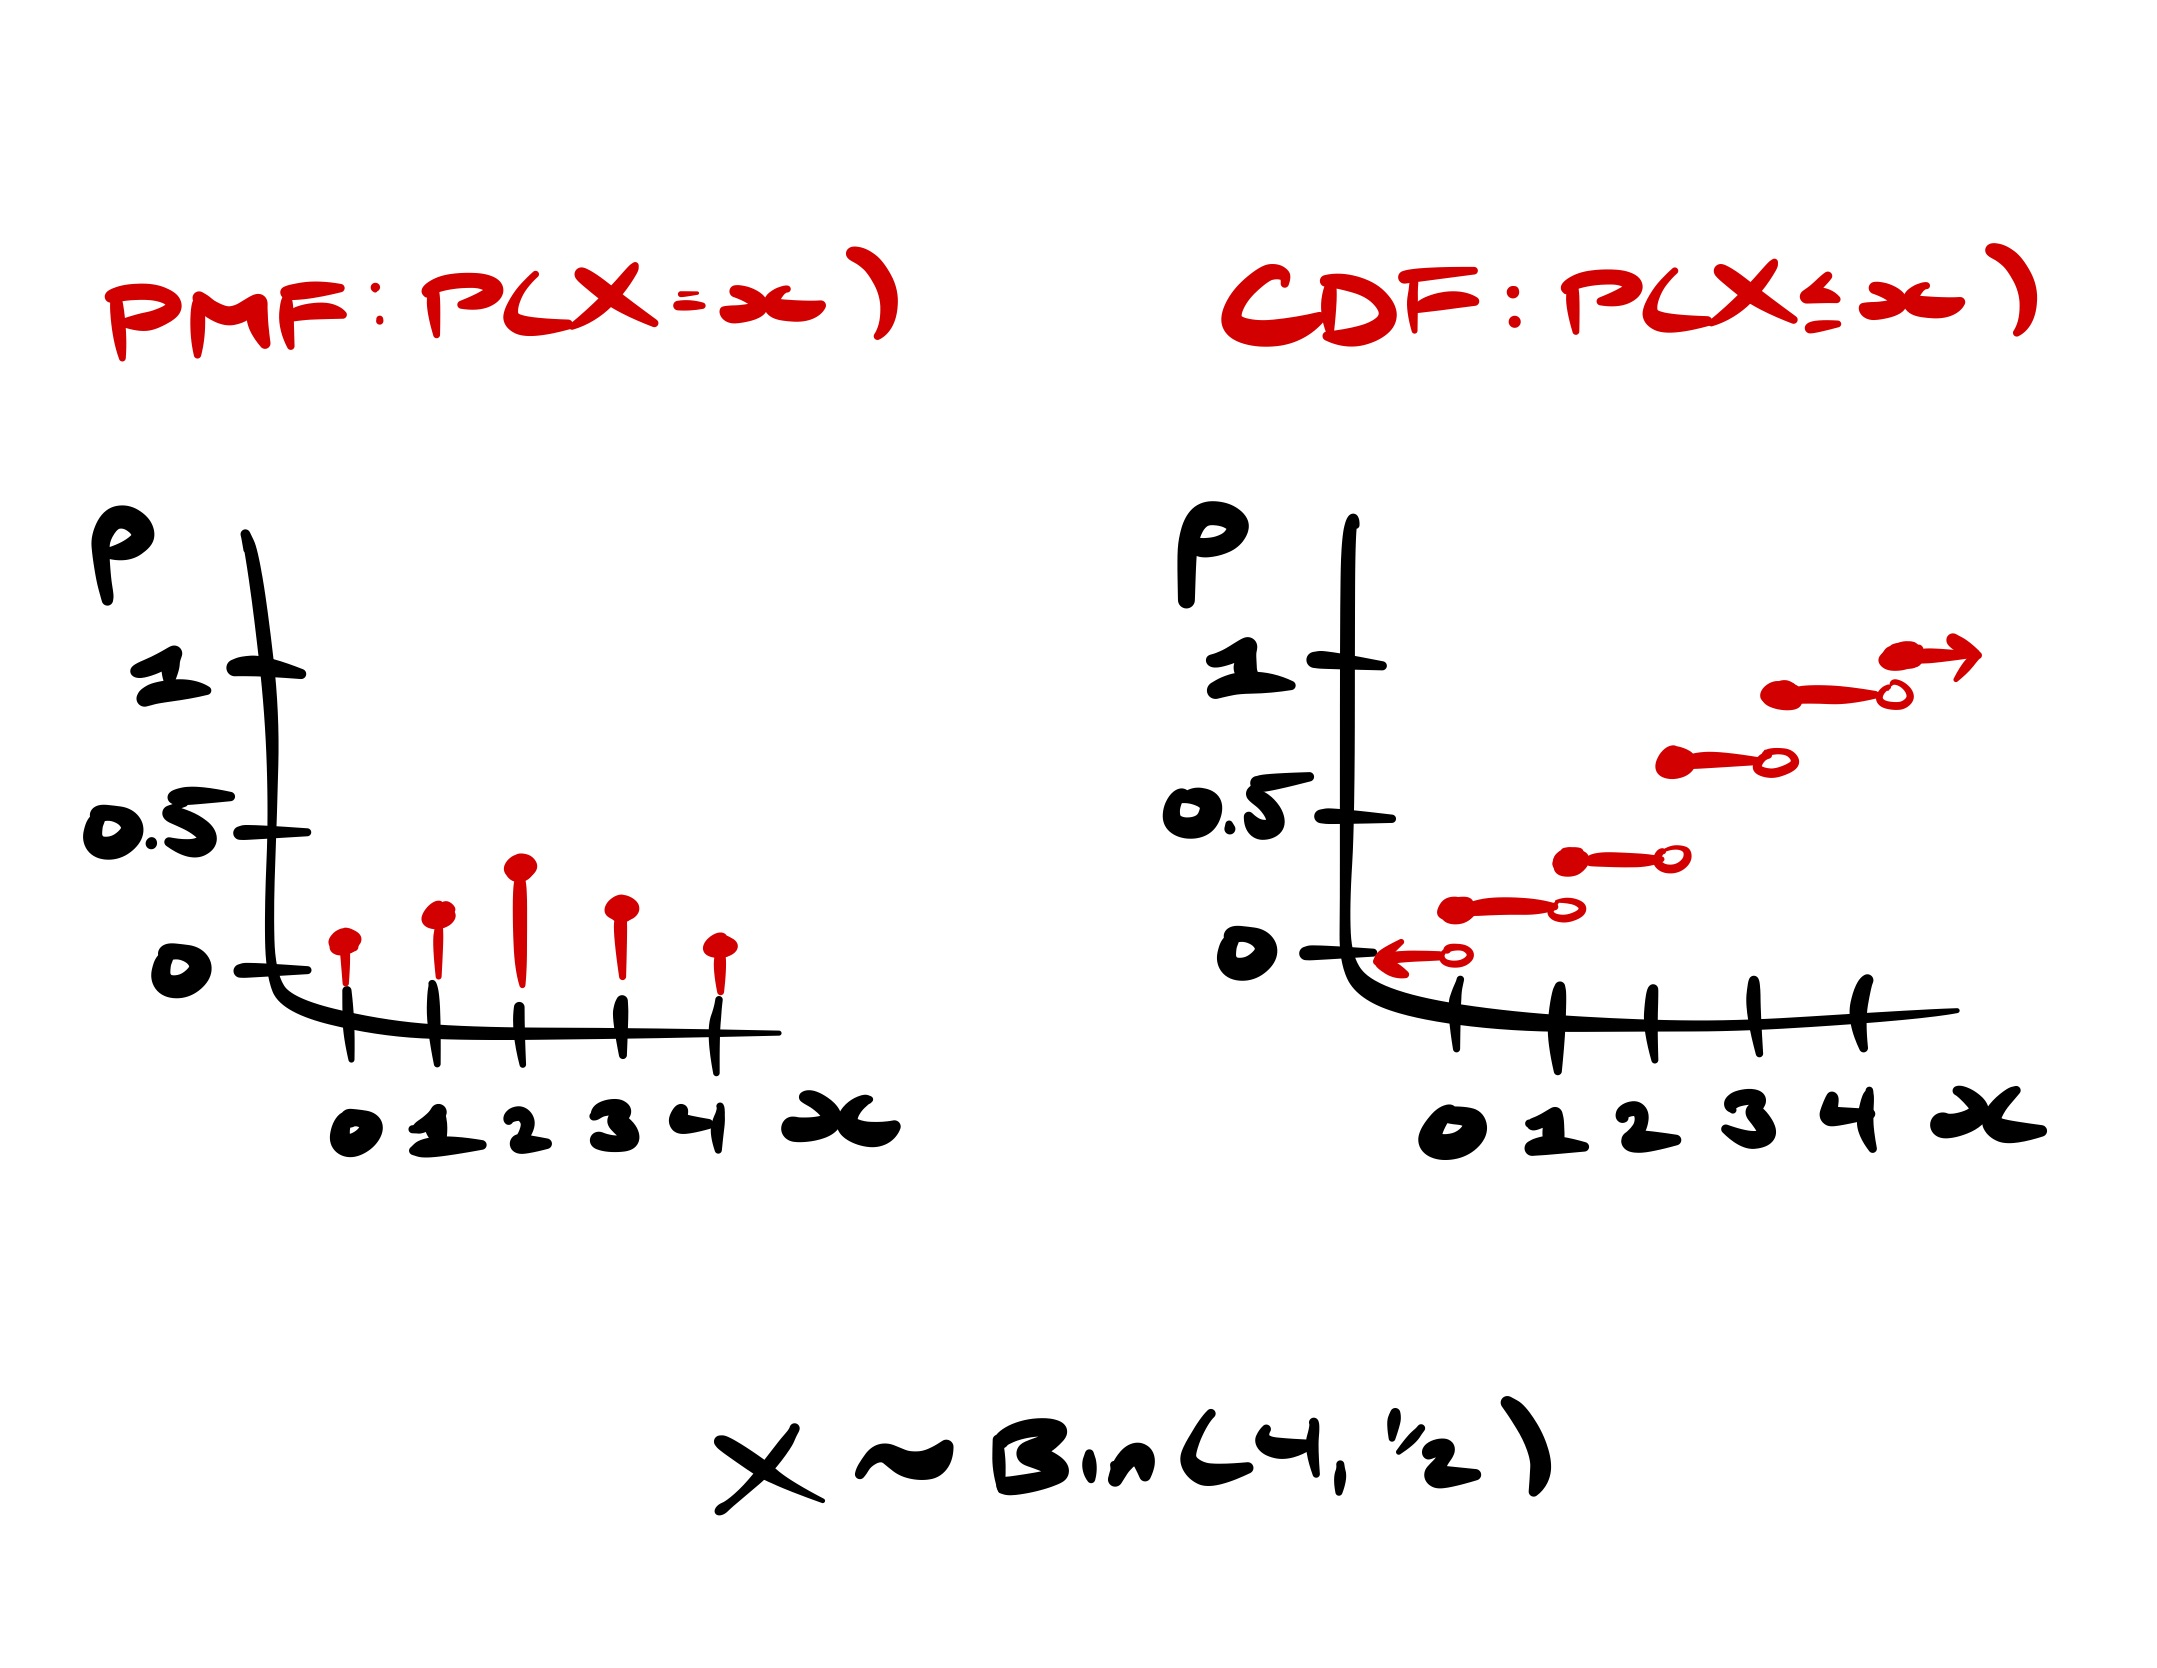
\includegraphics[width=0.5\textwidth]{stat110_section3_figure3.jpg}\\{\footnotesize FIGURE 3: The PMF and CDF for $X \sim \Bin(4, \frac{1}{2})$.}
\end{center}

\begin{definition}[Cumulative distribution function]
If $X$ is a random variable (discrete or continuous), then we can describe its distribution with \[F(x) = P(X \leq x),\] where $F(x)$ is the \textit{cumulative distribution function} (CDF).

$\bullet$ A CDF for $X$ with support $\{x_1, x_2, \ldots\}$ must satisfy the following criteria:

$\bullet$ \textbf{$F$ is nondecreasing}: If $x_1 \leq x_2$, then $F(x_1) \leq F(x_2)$.

$\bullet$ \textbf{Right-continuous}: For any $a$, we have $F(a) = \lim_{x \rightarrow a^+} F(x)$.

$\bullet$ \textbf{Convergence in the limits}: $\lim_{x \rightarrow \infty} F(x) = 1$ and $\lim_{x \rightarrow - \infty} F(x) = 0$.
\end{definition}

\begin{concept}
Let $X$ be a discrete random variable with CDF $F(x)$ and support $\mathbb{N}$. What is the CDF a function of? How can we find $P(X = 110)$ in terms of $F(x)$?
\end{concept}

\begin{solutionbox}
Like the PMF, the CDF is a function of possible crystallizations of $X$—e.g., $P(X \leq 0)$ vs. $P(X \leq 1)$—and outputs probabilities—i.e., $F: \R \rightarrow [0, 1]$. $F(x) = P(X \leq x)$, so $F(110) - F(109) = P(X \leq 110) - P(X \leq 109) = P(X = 110)$.
\end{solutionbox}

% Section: More Famous Distributions
\section{More Famous Distributions}

\begin{idea}
In addition to the \textit{Bernoulli} and \textit{Binomial}, there are other important \textit{famous distributions} that often appear in probability and statistics.
\end{idea}

\begin{definition}[Geometric]
Let $X$ be distributed \textit{Geometric} with parameter $p$—i.e., \[X \sim \Geom(p).\]

$\bullet$ \textbf{Story}: $X$ is the number of failures until we observe a success in independent trials that each have success probability $p$, \textit{not} counting that first success.

$\bullet$ \textbf{Example}: Let $X$ be the number of tails observed until the first heads if we repeatedly flip a fair coin. Then $X \sim \Geom(0.5)$.

$\bullet$ \textbf{PMF and Support}: \[P(X = x) = (1 - p)^{x} p\] for $x \in \{0, 1, \ldots\}$.
\end{definition}

\begin{definition}[First Success]
A different convention of the \textit{Geometric} distribution. Let $X$ be distributed \textit{First Success} with parameter $p$—i.e., \[X \sim \FS(p).\]

$\bullet$ \textbf{Story}: $X$ is the number of trials until we observe a success in independent trials that each have success probability $p$, \textit{counting} that first success.

$\bullet$ \textbf{Example}: Let $X$ be the number of flips until the first heads if we repeatedly flip a fair coin (including the flip that lands heads). Then $X \sim \FS(0.5)$.

$\bullet$ \textbf{PMF and Support}: \[P(X = x) = (1 - p)^{x - 1} p\] for $x \in \{1, 2, \ldots\}$.

$\bullet$ \textbf{Properties}: If $X \sim \Geom(p)$, then \[X + 1 \sim \FS(p).\]
\end{definition}

\begin{concept}
Why does the support of the First Success start with $1$?
\end{concept}

\begin{solutionbox}
In the most extreme case, the very first trial is a success, in which case the number of trials until we observe a success is $1$. Additionally, since $X \sim \Geom(p)$ has support $\{0, 1, \ldots\}$, we can add $1$ to every value: $\{1, 2, \ldots\}$.
\end{solutionbox}

\begin{definition}[Negative Binomial]
Let $X$ be distributed \textit{Negative Binomial} with parameters $r$ and $p$—i.e., \[X \sim \NBin(r, p).\]

$\bullet$ \textbf{Story}: $X$ is the number of failures until we observe the $r$th success in independent trials that each have success probability $p$, \textit{not} counting any successes.

$\bullet$ \textbf{Example}: Let $X$ be the number of tails observed until the $3$rd heads if we repeatedly flip a fair coin. Then $X \sim \NBin(3, 0.5)$.

$\bullet$ \textbf{PMF and Support}: \[P(X = x) = \binom{x + r - 1}{r - 1} p^{r} (1 - p)^{x}\] for $x \in \{0, 1, \ldots\}$.

$\bullet$ \textbf{Properties}: If $X_1, \ldots, X_r \simiid \Geom(p)$, then \[X_1 + \ldots + X_r \sim \NBin(r, p).\]
\end{definition}

\begin{concept}
Let $X \sim \NBin(1, p)$. What is another way to describe the distribution of $X$?
\end{concept}

\begin{solutionbox}
$X \sim \Geom(p)$, which follows by the story of the Geometric and the property of the Negative Binomial.
\end{solutionbox}

\begin{definition}[Hypergeometric]
Let $X$ be distributed \textit{Hypergeometric} with parameters $w$, $b$, and $n$—i.e., \[X \sim \HGeom(w, b, n).\]

$\bullet$ \textbf{Story}: $X$ is the number of \textit{desirable} objects in a sample if we draw $n$ objects, \textit{without replacement}, from a population with $w$ \textit{desirable} objects and $b$ \textit{undesirable} objects (with $w + b$ total objects).

$\bullet$ \textbf{Example}: We draw $3$ cards, one at a time without replacement, from a shuffled deck with $4$ aces and $48$ non-aces. Let $X$ be the number of aces drawn. Then $X \sim \HGeom(4, 48, 3)$.

$\bullet$ \textbf{PMF and Support}: \[P(X = x) = \frac{\binom{w}{x} \binom{b}{n - x}}{\binom{w + b}{n}}\] for $x \in \{\max(0, n - b), \ldots, \min(n, w)\}$.

$\bullet$ \textbf{Properties}: If $X \sim \Bin(n, p)$ and $Y \sim \Bin(m, p)$ with $X \indep Y$, then \[X \mid \{X + Y = r\} \sim \HGeom(n, m, r).\]
\end{definition}

\begin{concept}
Let $X \sim \HGeom(w, b, n)$. Derive the Hypergeometric PMF—i.e., $P(X = x)$—via story proof.
\end{concept}

\begin{solutionbox}
$X$ is the number of desirables in our sample, and let $x$ be an arbitrary crystallization. We can use naive probability because the sample space is finite and consists of equally likely outcomes. Thus, we want the number of favorable outcomes over the total number of outcomes. In the numerator, we choose our $x$ desirables out of the population's $w$ desirables and then choose our remaining $n - x$ undesirables out of the population's $b$ undesirables. There are $\binom{w + b}{n}$ total samples of size $n$, so $P(X = x) = \frac{\binom{w}{x}\binom{b}{n-x}}{\binom{w+b}{n}}$.
\end{solutionbox}

% Section: Exercises
\section{Exercises}

\begin{problem}
\textit{Thirteen} is a popular Vietnamese card game played with a standard $52$-card deck between $4$ players, who are each dealt $13$ cards. The cards are ranked from weakest to strongest—hearts are the strongest suit, and two is the strongest value. Players take turns playing combinations of cards, where each play has to beat the previous one based on ranking. The first player to get rid of all of their cards wins the game.

(a) Suppose that Alice, Bob, Charlie, and David want to play a round. In some versions of the game, a player who is dealt all $4$ twos immediately wins the round. What is the probability that this happens to Alice?

(b) We may be more interested in this event occurring for \textit{any} of the players, not just Alice. What is the probability that any player is dealt all $4$ twos?

(c) Now suppose that Alice, Bob, Charlie, and David play $13$ rounds, shuffling the deck before each round. What is the probability that Alice is dealt $2$ twos in $2$ of the rounds and in none of the other rounds?

(d) What is the probability that Alice is dealt $2$ twos in the \textit{first} $2$ rounds and in none of the other rounds?
\end{problem}

\begin{solutionbox}
(a) Let $X$ be the number of twos dealt to Alice in a round, with support $\{0, \ldots, 4\}$. By the story of the Hypergeometric, $X \sim \HGeom(4, 48, 13)$. By the Hypergeometric PMF, $P(\text{Alice is dealt all 4 twos}) = P(X = 4) = \frac{\binom{4}{4} \binom{48}{9}}{\binom{52}{13}} = 0.00264$. This makes sense by naive probability. Being dealt $4$ twos is the same event as being dealt $9$ non-twos. There are $\binom{52}{13}$ total ways to draw $13$ from the $52$ cards, and the number of favorable outcomes is $\binom{48}{9}$ (i.e., the number of ways to draw $9$ of the $48$ non-twos). 

(b) What we calculated in (a) applies to each player (i.e., replace Alice with Bob, and everything still holds). This is an argument of symmetry since all players are treated the same at first. Additionally, this event can only happen to 1 player maximum (i.e., mutual exclusion). Thus, we can multiply the probability in (a) by $4$ for the $4$ different players who could have this happen, so $P(\text{any player is dealt all 4 twos}) = 4 \times 0.00264 = 0.01056$. More formally, $P(\text{this happens to any player}) = P(\text{this happens to Alice} \cup \ldots \cup \text{this happens to David}) = P(\text{this happens to Alice}) + \ldots + P(\text{this happens to David}) = 4 \times P(\text{this happens to Alice})$.

(c) Let $Y$ be the number of rounds where Alice is dealt $2$ twos. With $X$ defined in (a), $P(\text{Alice is dealt 2 twos in a round}) = P(X = 2) = \frac{\binom{4}{2} \binom{48}{11}}{\binom{52}{13}} = 0.21349$. By the story of the Binomial, $Y \sim \Bin(13, 0.21349)$. By the Binomial PMF, $P(\text{Alice is dealt 2 twos in 2 of the rounds}) = P(Y = 2) = \binom{13}{2} 0.21349^{2} (1 - 0.21349)^{13 - 2} = 0.25327$.

(d) From before, $P(\text{Alice is dealt 2 twos in a round}) = 0.21349$. By the multiplication rule, $P(\text{Alice is dealt 2 twos in the first 2 rounds and in none of the other rounds}) = 0.21349^{2} (1 - 0.21349)^{11} = 0.00324$. Notice we're not using the Binomial distribution anymore. Before, we were interested in successes in \textit{any} $2$ rounds (so the $\binom{13}{2}$ term accounts for the different permutations possible). Now, we're specifying which of the trials have to be successes (specifically, the first $2$).
\end{solutionbox}

\begin{problem}
\textit{Rock, Paper, Scissors} is a simple hand game played by $2$ players, who simultaneously choose $1$ of $3$ options: rock, paper, or scissors. Rock defeats scissors, scissors defeats paper, and paper defeats rock (if both players choose the same option, the round ends in a tie). 

(a) Suppose that Alice and Bob want to play, and they do so randomly (i.e., for each round, all outcomes are equally likely). What is the probability that Alice wins a round?

(b) In practice, we usually ignore ties and only look at \textit{decisive} rounds (i.e., those that end in a win or loss). What is the probability that Alice wins a decisive round?

(c) Now suppose that Alice and Bob play a \textit{best of 7} series (i.e., the first person to win 4 decisive rounds wins the series). Additionally, let $p$ be the probability that Alice wins a decisive round, allowing us to generalize to other games with a best of $7$ series. What is the probability that Alice wins the series? What happens if $p = \frac{1}{2}$?
\end{problem}

\begin{solutionbox}
(a) $P(\text{Alice wins a round}) = \frac{1}{3}$. This is an argument of symmetry (i.e., each of the 3 options for Alice—win, tie, loss—are equally likely). However, we can also reason through this via counting and naive probability. We are sampling $k = 2$ from $n = 3$ with replacement and where order matters. Of the $3^2 = 9$ outcomes, 3 of them—$\{R, S\}, \{S, P\}, \{P, R\}$—are favorable for Alice to win the round.

(b) Using the same arguments as (a) but adjusting for the new sample space, $P(\text{Alice wins a decisive round}) = \frac{1}{2}$.

(c) $P(\text{Alice wins the series}) = \sum_{x = 4}^{7} \binom{7}{x} p^{x} (1 - p)^{7 - x}$. An elegant solution is to assume that Alice and Bob play all 7 decisive rounds no matter what. Let $X$ be the number of those where Alice wins, with support $\{0, \ldots, 7\}$. By the story of the Binomial, $X \sim \Bin(7, p)$, so $P(\text{Alice wins the series}) = P(X \geq 4) = P(X = 4) + P(X = 5) + P(X = 6) + P(X = 7) = \sum_{x = 4}^{7} \binom{7}{x} p^{x} (1 - p)^{7 - x}$ using the Binomial PMF. If $p = \frac{1}{2}$, $P(\text{Alice wins the series})$ simplifies to $\frac{1}{2}$. This makes sense intuitively; with random play, neither player should have an advantage. This solution can feel off if the series can be decided before $7$ games (e.g., if Alice wins the first $4$ games). Why does the answer not depend on whether the teams play all $7$ games? Imagine telling Alice and Bob to continue playing even after the overall winner has been decided (just for fun). The actual outcome of the series wouldn't be affected by this, which means that the probability that Alice wins the match wouldn't be affected, either!
\end{solutionbox}

\end{document}